\cleardoublepage
\chapter{Global characterisation of isoform diversity in the mouse cortex}
\label{ch: whole_transcriptome}

%While the methods I have adopted for long-read sequencing in this thesis allows interrogation of full-length transcripts, this is reliant on the generation and amplification of cDNA from mRNA, which can produce artefacts (template switching), introduce bias (distortion of relative cDNA abundance) and lose RNA modifications. In 2018, ONT showed that it was able to sequence RNA directly using the minION by adding poly(T) adapters directly to the mRNA, with a translocase that was able to bind and process RNA efficiently	 \cite{Garalde2018}, achieving coverage and accuracy comparable to that with ONT-cDNA method. 

% Recite
This chapter is an abridged and modified version of a peer-reviewed manuscript, which I co-authored and has been accepted for publication in Cell Reports (Leung et al. 2021)\cite{Leung2021} (the complete published paper is presented in \textbf{\cref{app_cell}}). Additional lab QC output and run reports are included. 

\section{Introduction}
Characterisation of the full complement of isoforms across tissues and development is important for understanding the role of transcriptional variation in health and disease. Previous transcriptomic profiling studies of AD post-mortem brain tissue and AD mouse models have revealed significant variation in transcript expression and splicing (reviewed in \cref{tab: AS_ADHuman_studies} and \cref{tab: AS_ADMouse_studies}, respectively), implicating the role for transcriptomic dysregulation and aberrant splicing in AD pathogenesis\cite{Raj2018}. Despite significant advances in sequencing technology, the accurate detection of alternative splicing events and isoform diversity remains a challenge due to technical limitations with standard RNA-Seq approaches (explained in \cref{rnaseq_intro}). Recent advances in long-read cDNA sequencing address these limitations - Pacific Biosciences (PacBio) Isoform Sequencing (Iso-Seq) and Oxford Nanopore Technologies (ONT) nanopore sequencing (described in \cref{sec:pb_isoform_sequencing} and \cref{sec:ONT_cDNA_Sequencing}, respectively) - enabling direct assessment of alternatively-spliced transcripts\cite{Amarasinghe2020}.

\newpage
Given the importance to comprehensively characterise the full complement of isoforms, this chapter aimed to characterise the global isoform diversity and splicing events in the mouse cortex. The objectives of this chapter were as follows:
\begin{enumerate}
	\item To perform PacBio Iso-Seq profiling (as described in \cref{sec:pb_isoform_sequencing}) of the mouse cortex and generate full-length cDNA sequences. 
	\item To comprehensively annotate the mouse transcriptome and identify novel transcripts, novel genes and fusion genes.  
	\item To compare the performance of long-read Iso-Seq and short-read RNA-Seq for transcriptome annotation. 
	\item To comprehensively characterise splicing events in the mouse cortex.  	
\end{enumerate} 

\section{Methods}
\subsection{Samples}
Entorhinal cortex tissue was dissected from 6 female rTg4510 transgenic mice and 6 wild-type mice, aged 2 and 8 months (n = 3 mice per group) (\cref{tab:whole_phenotype}). Additional details on mouse breeding conditions and animal procedures can be found in \cref{sec: animalbreeding_sample preparation}. For each mouse sample, RNA was isolated using the AllPrep DNA/RNA Mini Kit (Qiagen) from \textasciitilde5mg tissue and quantified using the Bioanalyzer 2100 (Agilent) (described in \cref{section:ch2_bioanalyzer}). 

\subsection{Iso-Seq library preparation and SMRT sequencing}\label{ch4_methods: isoseq_library}
RNA from each mouse sample was prepared for Iso-Seq library preparation and SMRT sequencing following the Iso-Seq lab workflow, as detailed and described in \cref{chap:isoseq_labpipeline}. Briefly, first-strand cDNA synthesis was performed on 200ng RNA using the SMARTer PCR cDNA Synthesis Kit (Clontech) (described in \cref{section:ch2_cDNA_synthesis_explanation}), with the addition of External RNA Controls Consortium (ERCC) standards to the majority of mouse cortex samples (n = 10) (described in \cref{section:ch2_ERCC_explanation}), followed by PCR amplification of 14 cycles with PrimeSTAR GXL DNA Polymerase (Clontech) (described in \cref{section:ch2_PCR_explanation}); an example of an agarose gel image taken after PCR amplification is provided in \cref{fig:isoseq_whole_pccresults}. The resulting amplicons were then divided into two fractions and purified using 0.4X and 1X AMPure PB beads (as shown in \cref{fig:isoseq_whole_bioresults}). The two fractions were then recombined at equimolar quantities and library preparation was performed using the SMRTbell Template Prep Kit v1.0 (shown in \cref{fig:isoseq_whole_bioresults}). Each sample was then sequenced on the PacBio Sequel 1M SMRT cell with the v3 chemistry (Diffusion Loading at 5pM with a 4-hour pre-extension and a 20-hour capture time) (described in \cref{section:ch2_sequencing}).

\vspace{1cm}
\begin{table}[h]
    \setlength\tabcolsep{7pt} %reduced margin size in table
	\captionsetup{width=0.95\textwidth}
	\caption[Phenotype information of the mouse samples used for global transcriptome profiling]%
	{\textbf{Phenotype information of the mouse samples used for global transcriptome profiling.} Tabulated is a summary of the phenotype information of the rTg4510 mouse samples sequenced using Iso-Seq and RNA-Seq.\newline ECX - Entorhinal cortex, ONT - Oxford Nanopore Technologies, RIN - RNA integrity number, TG - Transgenic rTg4510 mice, WT - Wild-type.}
	\label{tab:whole_phenotype}
	\centering
	\begin{tabular}{@{}cccccccc@{}}
		\toprule
		Sample ID & Tissue & Sex & Genotype & Age (months) & RIN & Iso-Seq & RNA-Seq  \\ \midrule
		Mouse 1   & ECX    & F   & WT       & 2         & 9.2 & \checkmark       &  \checkmark         \\
		Mouse 2   & ECX    & F   & TG       & 2         & 8.8 & \checkmark        & \checkmark        \\
		Mouse 3   & ECX    & F   & WT       & 8         & 9.1 & \checkmark        & \checkmark        \\
		Mouse 4   & ECX    & F   & TG       & 8         & 9.2 & \checkmark        & \checkmark        \\
		Mouse 5   & ECX    & F   & TG       & 8         & 8.7 & \checkmark        & \checkmark        \\
		Mouse 6   & ECX    & F   & WT       & 2         & 9.2 & \checkmark        & \checkmark        \\
		Mouse 7   & ECX    & F   & TG       & 2         & 8.9 & \checkmark        & \checkmark        \\
		Mouse 8   & ECX    & F   & WT       & 8         & 9   & \checkmark        & \checkmark       \\
		Mouse 9   & ECX    & F   & TG       & 8         & 8.6 & \checkmark        & \checkmark        \\
		Mouse 10  & ECX    & F   & WT       & 2         & 9.2 & \checkmark        & \checkmark        \\
		Mouse 11  & ECX    & F   & TG       & 2         & 8.9 & \checkmark        & \checkmark       \\
		Mouse 12  & ECX    & F   & WT       & 8         & 9.1 & \checkmark        & \checkmark        \\ \bottomrule
	\end{tabular}
\end{table}

\vspace{1cm}
\begin{figure}[!htp]
	\centering
	\includegraphics[page=2,trim={2.5cm 25cm 0cm 0cm},clip,scale = 1]{Figures/WholeTranscriptome_Figures.pdf}
	\captionsetup{width=0.95\textwidth}
	\caption[Iso-Seq global transcriptome profiling - PCR cycle optimisation]%
	{\textbf{Samples were amplified using 14 PCR cycles.} Shown is an example of an agarose gel image from PCR cycle optimisation of four mouse samples after cDNA synthesis. PCR aliquots were collected every two cycles (10, 12, 14, 16, 18, 20) and then assayed using agarose gel electrophoresis. 14 cycles were determined to be optimum for large-scale amplification, as cycles below showed insufficient amplification whereas cycles above showed signs of over-amplification, which could result in a biased sequencing representation. Ladder (L) denotes to a 1kb DNA ladder.}
	\label{fig:isoseq_whole_pccresults}
\end{figure}

\begin{figure}[!htp]
	\centering
	\vspace{20pt}
	\includegraphics[page=3,trim={1cm 12cm 0 0cm},clip,scale = 0.8]{Figures/WholeTranscriptome_Figures.pdf}
	\captionsetup{width=0.95\textwidth}
	\caption[Iso-Seq global transcriptome profiling - SMRTbell library preparation]%
	{\textbf{Library preparation was performed for each sample with successful cDNA purification and ligation with SMRT bell templates.} Following large-scale amplification using the optimal cycle number (as determined from \cref{fig:isoseq_whole_pccresults}), the resulting cDNA was divided into two fractions (denoted here as F1 and F2) and purified using 1X (F1) and 0.4X (F2) AMPure beads. Shown is \textbf{(A)} a Bioanalyzer gel of the purified cDNA from the two fractions, and zoomed-in Bioanalyzer electropherograms of \textbf{(B)} Mouse 1 Fraction 1, \textbf{(C)} Mouse 1 Fraction 2, \textbf{(D)} Mouse 1 and \textbf{(E)} Mouse 8 after library preparation. The x-axis of the Bioanalyzer electropherogram represents the molecular size. Size distribution for each fraction was determined from the start to the end point of the smear. 
	\\
	\\	 	
	Of note, cDNA in Fraction 2 has a significantly higher molecular weight across all the samples as expected (shown in Figures A and C). Pooling of both fractions enriched for higher molecular weight cDNA molecules, which were intact after performing SMRTbell template preparation (as seen in Figures D and E). Despite the fact that samples were prepared sequentially, Bioanalyzer electropherogram profiles were fairly consistent across samples. 
	}
	\label{fig:isoseq_whole_bioresults}
\end{figure}

\clearpage
\subsection{RNA-Seq library Preparation and Illumina sequencing}
RNA from the same mouse samples (n = 12) was processed in parallel using the TruSeq Stranded mRNA Sample Prep Kit (Illumina) and subjected to 125bp paired-end sequencing using the HiSeq2500 (Illumina)\cite{Castanho2020}. Briefly, cDNA libraries were prepared from \textasciitilde450ng of total RNA plus ERCC spike-in synthetic RNA controls (Ambion, dilution 1:100), purified using AMPure XP magnetic beads (Beckman Coulter) and profiled using the D1000 ScreenTape System (Agilent). 

\subsection{SMRT sequencing QC and Iso-Seq data processing}\label{ch4_methods: isoseq_data}
Raw Iso-Seq reads were evaluated using the SMRT Link Portal v7.0 and analysed using the optimised Iso-Seq bioinformatics pipeline, as depicted in \cref{fig:isoseq_whole_pipeline}. Further details are provided in \cref{section:isoseq_bioinformatics}. Briefly, CCS reads were generated from a minimum of 1 pass using \textit{Iso-Seq3 CCS} (v3.4.1). Primers and SMRT adapters were then removed using \textit{Lima} (v1.9) to generate full-length reads, followed by removal of artificial concatemers reads and trimming of poly(A) tails in \textit{Iso-Seq3 Refine}. Full-length, non-chimeric (FLNC) reads were then collapsed to high-quality transcripts using \textit{Iso-Seq3 Cluster}, and mapped to the mouse reference genome (mm10) using \textit{Minimap2} (v2.17) with the following parameters “-ax splice -uf --secondary=no -C5 -O6,24 -B4”. \textit{ Cupcake collapse-isoforms-by-sam.py} script was subsequently applied with the following parameters  “-c 0.85 -i 0.95 --dun-merge-5-shorter” to reduce redundancy. 

\subsection{Transcriptome annotation and filtering}
\label{ch4: transcriptome_annotation}
After filtering for partial isoforms (such as 5’ degradation products) using \textit{TAMA} with default parameters, isoforms detected using SMRT sequencing were characterized and classified using \textit{SQANTI2} (v7.4) in combination with mouse reference gene annotations (mm10, GENCODE, vM22) , FANTOM5 CAGE peaks, poly(A) motifs, STAR output junction file, full-length read counts (abundance file), and \textit{Kallisto}-derived counts from RNA-Seq data (described below in \cref{ch4: rnaseq_processing}). Additional details are provided in \cref{section: sqanti_annotations}. Potential artefacts such as reverse transcription jumps or intra-priming of intronic lariats were filtered out using the \textit{SQANTI2} filter script with an intra-priming rate of 0.6 (the fraction of genomic A's above which the isoform will be filtered, as detailed in \cref{section: sqanti_annotations}). The occurrence of mutually exclusive exons (MX) and exon skipping (ES) were assessed using \textit{SUPPA2}\cite{Trincado2018} with the parameter “–f ioe”, intron retention (IR) using \textit{SQANTI2}, and alternative first exons (AF), alternative last exons (AL), alternative 5’ splice sites (A5), and alternative 3’ splice sites (A3) using custom scripts based on splice junction coordinates. 

\subsection{RNA-Seq QC and data processing}
\label{ch4: rnaseq_processing}
Raw RNA-Seq reads were filtered (removal of ribosomal sequences, quality threshold of Q20, minimum sequence length of 35bp) and trimmed using \textit{fastqmcf} (v1.0), yielding a mean trimmed read depth of \textasciitilde20 million reads per sample. Reads were then mapped to the mouse reference genome (mm10) using \textit{STAR}\cite{Dobin2013} (v1.9). Gene and transcript expression were determined by aligning merged RNA-Seq reads to the Iso-Seq derived annotations (\textit{Cupcake} collapsed) using \textit{Kallisto}\cite{Bray2016} (v0.46.0) with default parameters. An RNA-Seq derived annotation was also generated from RNA-Seq reads and the mouse reference annotation (mm10, GENCODE, vM22) using \textit{Stringtie}\cite{Pertea2015} (v2.1.4), which was subsequently annotated and filtered using \textit{SQANTI2} under default parameters. 

\begin{figure}[htp]
	\centering
	\vspace{20pt}
	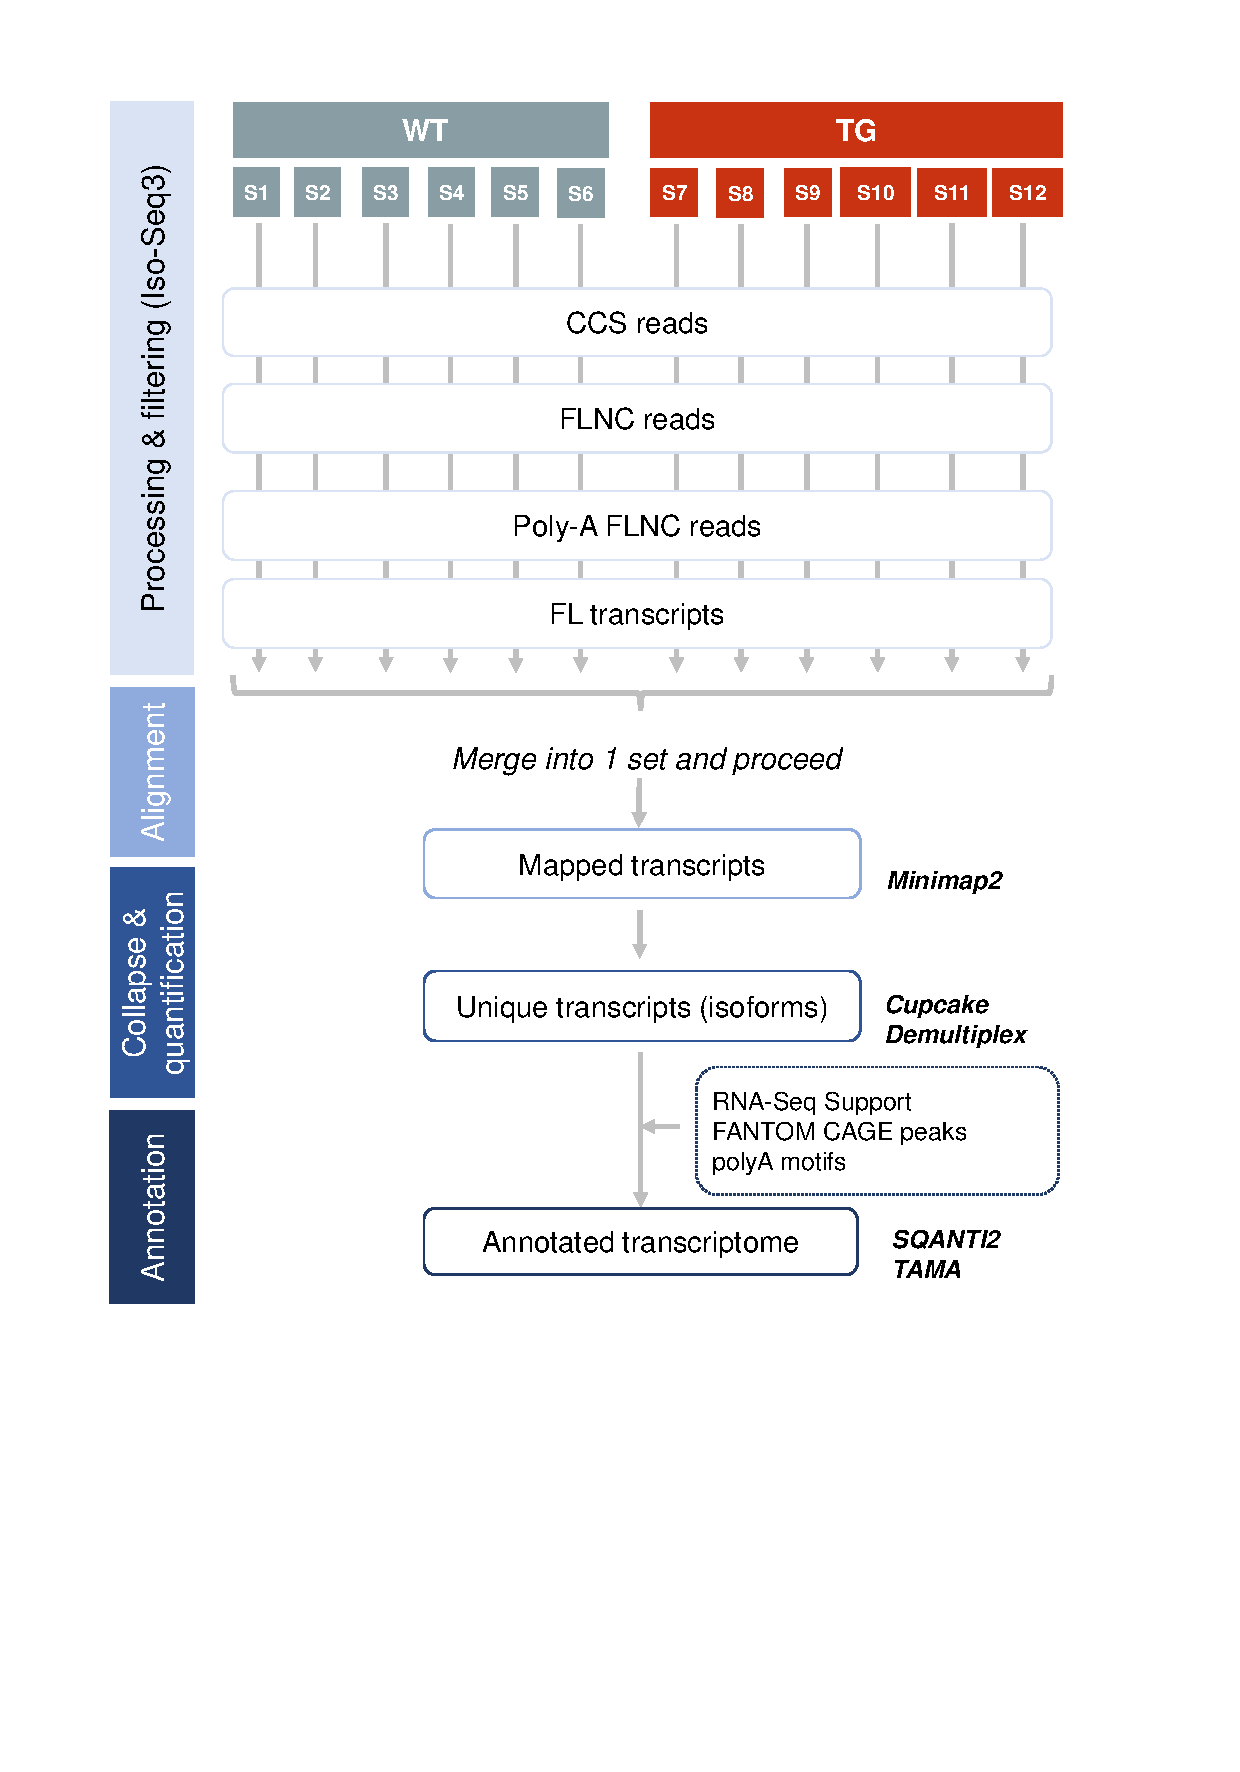
\includegraphics[page=1,trim={0 7cm 2cm 1cm},clip, scale = 0.7]{Figures/WholeTranscriptome_Figures.pdf}
	\captionsetup{width=0.95\textwidth}
	\caption[Detailed Iso-Seq bioinformatics pipeline for global transcriptome profiling]%
	{\textbf{Iso-Seq reads from each mouse sample were processed individually before merging into one unified dataset.} Shown is an overview of the bioinformatics pipeline used to generate full-length transcript annotations of the mouse entorhinal cortex (n = 12, WT = 6, TG = 6). Briefly, polymerase reads generated from PacBio Sequel I for each sample were processed using \textit{Iso-Seq3} (v3.1.2) and \textit{Cupcake} to generate high quality, full-length transcripts, which were then mapped to the mouse reference genome using \textit{Minimap2}. Isoforms were then collapsed and merged to generate one complete dataset, which was annotated using \textit{SQANTI2}. Additional details can be found in \cref{section:isoseq_bioinformatics}. CCS - Circular consensus sequence, FLNC - Full-length non-chimeric, FL - Full-length.}
	\label{fig:isoseq_whole_pipeline}
\end{figure}
 
\newpage
\section{Results}

\subsection{PacBio Iso-Seq run performance and sequencing metrics}
Following library preparation and SMRT sequencing, we generated a total of 371Gb (s.d = 4.35Gb, range = 22.5Gb - 38.7Gb) and 8,082,647 polymerase reads (s.d = 63,013 reads, range = 530,974 - 733,495 reads) (\cref{tab:isoseq_wholerun_result}). Following the Iso-Seq bioinformatics pipeline, raw reads were processed and clustered to unique consensus transcripts, which were then mapped to the genome. A total of 5.66 million CCS reads (sample mean = 471K, s.d = 46.8K, range =  353K - 512K) and 4.5 million FLNC reads were successfully generated (sample mean = 379K, s.d = 47.0K, range = 270K - 412K). Clustering of these reads yielded a total of \textasciitilde273K high-quality full-length transcripts (97\% of all FL transcripts, mean = 32.7K, s.d = 1.25K, range = 30.3K - 34.4K), which were mapped to 278K loci of the mouse reference genome (5K had multi-mapping). After filtering for alignment length and identity (described in \cref{ch4_methods: isoseq_data}), 266K transcripts were retained. Rarefaction curves confirmed that the dataset approached saturation, indicating that our coverage of the isoform diversity was representative of the true population of transcripts (\cref{fig:isoseq_whole_rarefaction}\textbf{A}). 

\subsection{Widespread isoform diversity in the mouse cortex}
Following stringent quality-control, Iso-Seq reads mapped to 14,482 known genes with expression patterns reflecting those expected for the cortex; using the Mouse Gene Atlas database, the 500 most abundantly-expressed genes were most significantly enriched for the “cerebral cortex” (odds ratio = 6.07, adjusted \textit{P} = 6.8 x 10\textsuperscript{-17}). We identified 46,626 isoforms (mean length = 3.18kb, s.d = 1.68kb, range = 0.083 – 15.9kb), which were enriched near Cap Analysis Gene Expression (CAGE) peaks from the FANTOM5 dataset (median distance from CAGE peak = -1bp, 35,262 (75.6\%) transcripts located within 50bp of a CAGE peak), and were also located proximal to annotated transcription start sites and transcription termination sites. A significant proportion of isoforms (n = 20,621, 45\%) were sized 2 - 4kb in length (median length = 2.96kb, mean length = 3.18kb, s.d = 1.68kb, range = 0.083kb - 15.9kb) (\cref{fig:isoseq_whole_rarefaction}\textbf{B}), corresponding to the mean length of mRNA in the mouse reference genome, with a wide range in the number of exons (range = 1 - 89) observed per isoform (mean number of exons = 10.8). A wide range in the number of multi-exonic RNA isoforms was also identified per gene (range = 1 - 86), and longer genes with more exons were typically annotated with more isoforms (Pearson's correlation between isoform number and gene length: corr = 0.25, \textit{P} = 1.33 x 10\textsuperscript{-197}; Pearson's correlation between isoform number and exon number: corr = 0.25, \textit{P} = 4.02 x 10\textsuperscript{-193}). Notably, only 10\% of isoforms (n = 4,641) were detected across all the samples (\cref{fig:isoseq_whole_lowlyexp}\textbf{A}), with about half (47.8\%) detected in 2 - 3 samples with very low transcript expression (\cref{fig:isoseq_whole_lowlyexp}\textbf{B}). 

\vspace{1cm}
\begin{figure}[!h]
	\begin{center}
		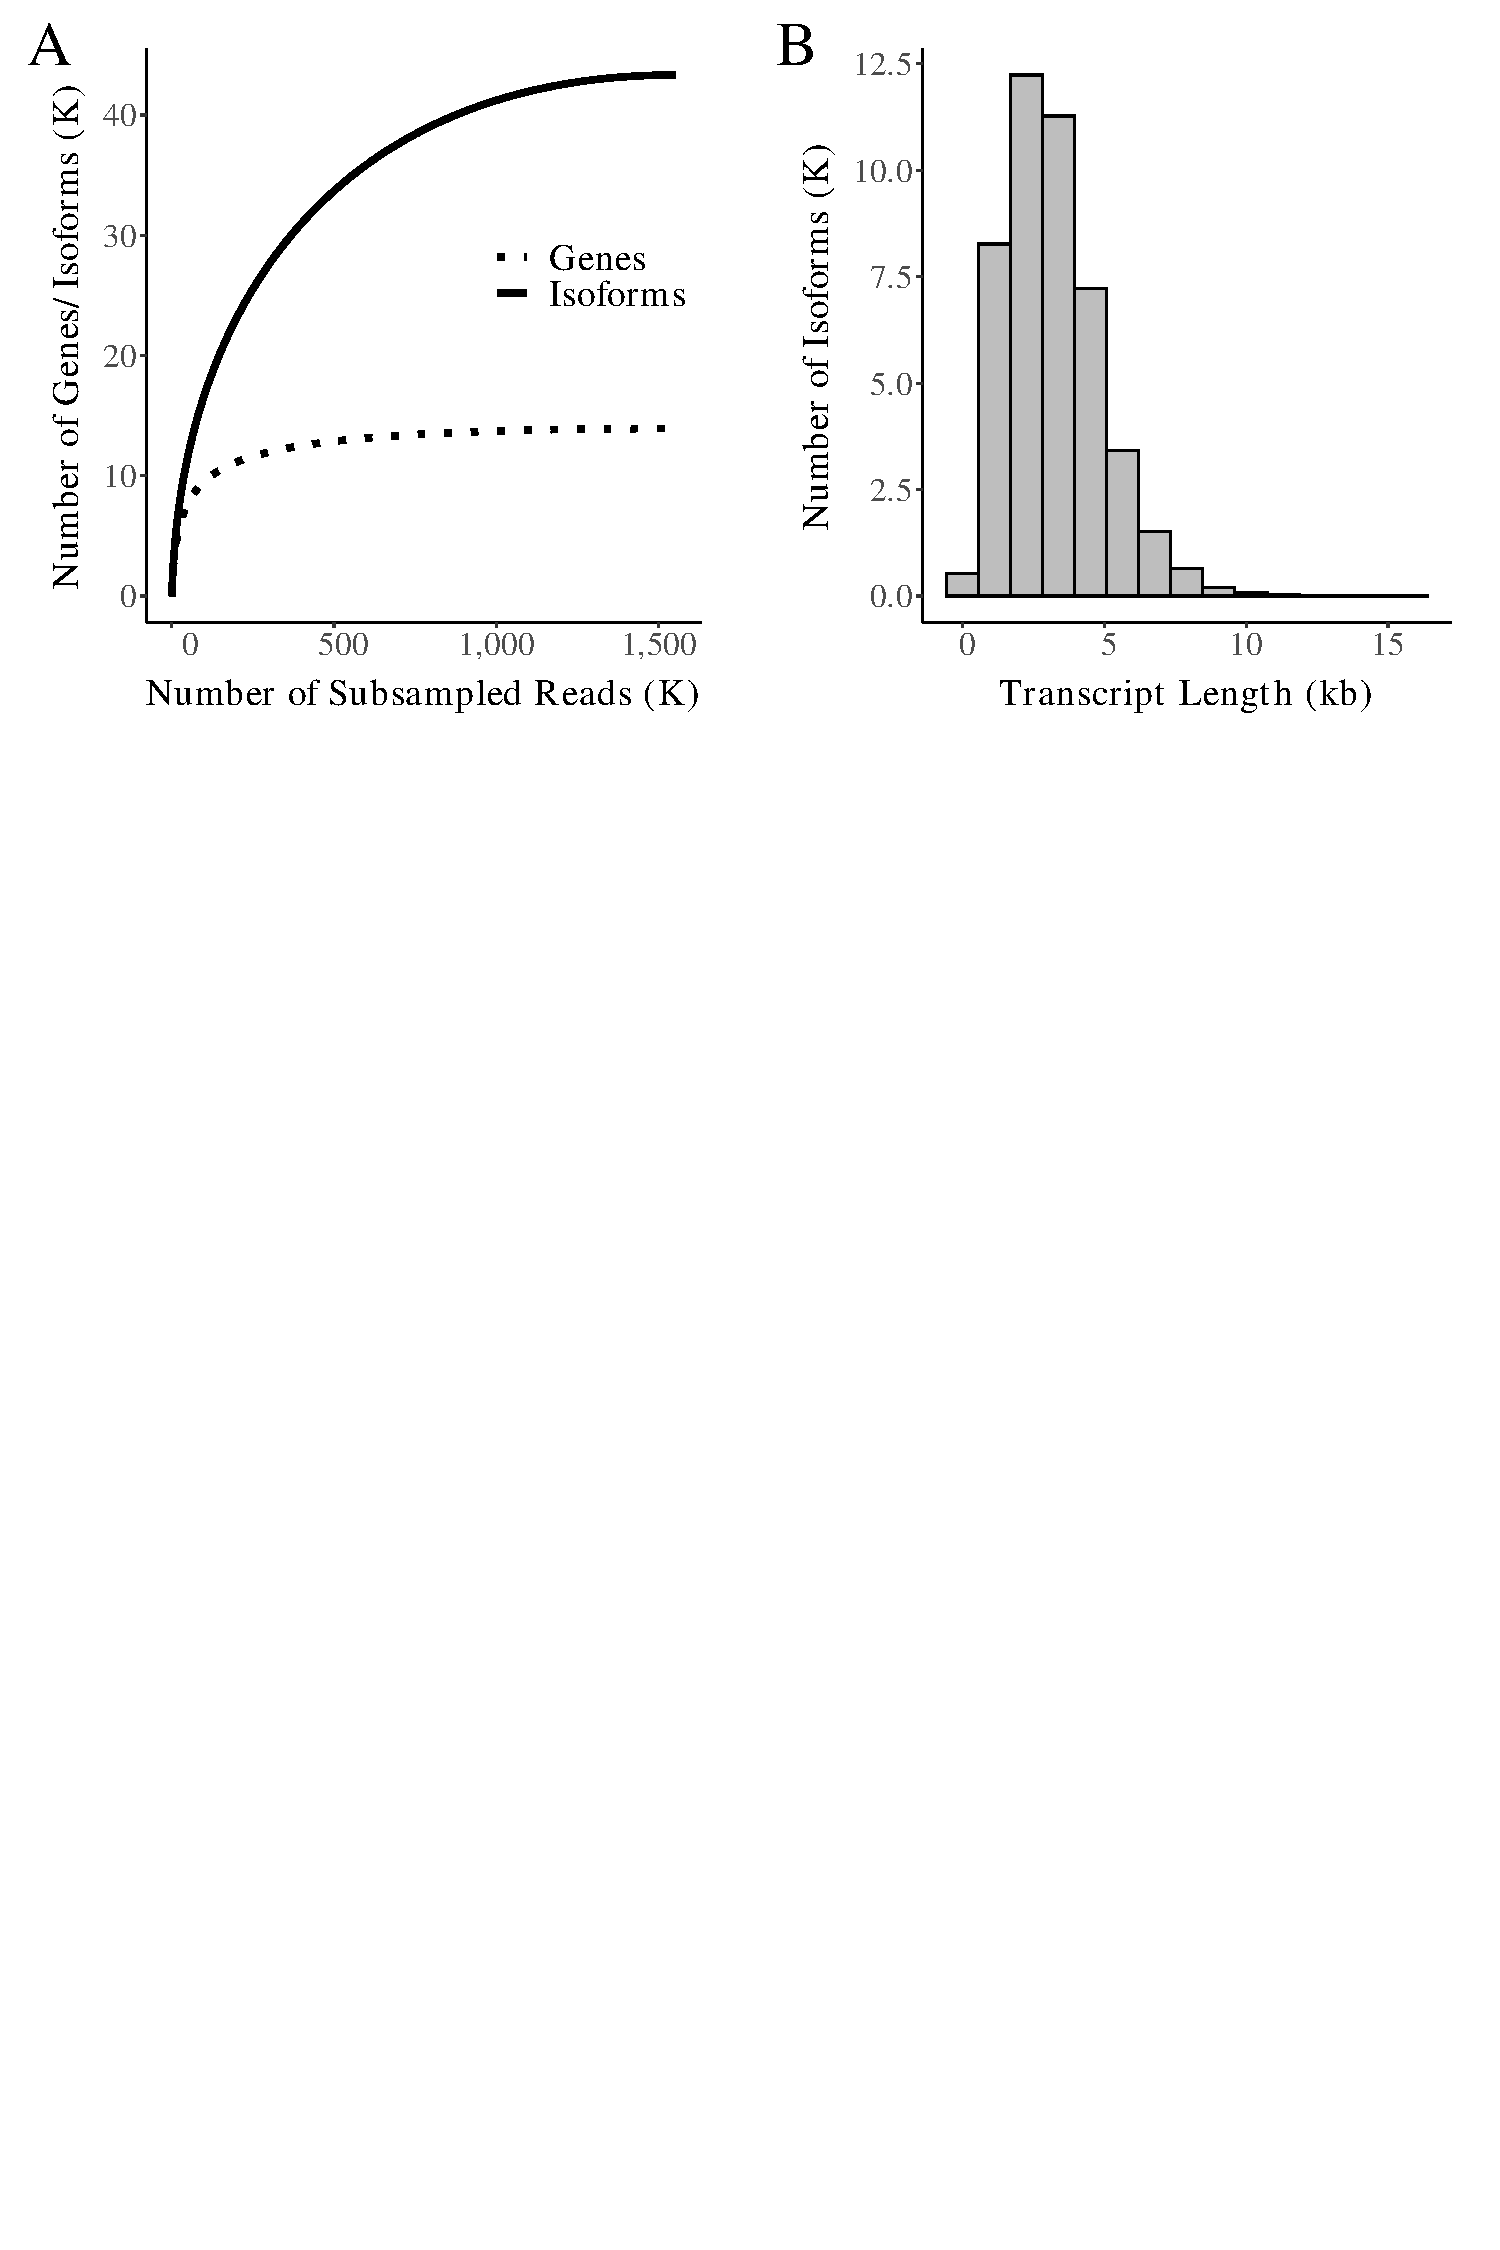
\includegraphics[page=1,trim={0 26cm 0 0},clip,scale = 0.55]{Figures/IsoSeqWholeTranscriptome.pdf}
	\end{center}
	\captionsetup{width=0.95\textwidth}
	\caption[Rarefaction curves from global transcriptome profiling of the rTg4510 cortex]%
	{\textbf{Saturation was reached at the gene and isoform level with the majority of transcripts sized \textasciitilde3kb.} Shown is \textbf{(A)} a rarefaction curve of the number of subsampled reads against the number of unique genes and isoforms detected, and \textbf{(B)} a distribution of the transcript length from merging all the Iso-Seq datasets. K - Thousand.}
	\label{fig:isoseq_whole_rarefaction}
\end{figure}

\vspace{1cm}
\begin{figure}[!h]
	\begin{center}
		\includegraphics[page=2,trim={0 26cm 0 0},clip,scale = 0.55]{Figures/IsoSeqWholeTranscriptome.pdf}
	\end{center}
	\captionsetup{width=0.95\textwidth}
	\caption[Isoform diversity across the samples from global transcriptome profiling]%
	{\textbf{Highly-expressed isoforms were more likely to be sequenced across samples.} Shown is \textbf{(A)} the distribution of isoforms detected in the number of mouse samples, with a third detected in any two of the total 12 samples. However, \textbf{(B)} quantification of these isoforms had very low expression (1 - 2 FL reads), whereas those that were commonly detected across all 12 samples were more abundant. FL - Full-length.}
	\label{fig:isoseq_whole_lowlyexp}
\end{figure}

\newgeometry{left=2.7cm,bottom=1.5cm, right=1.5cm, top=1.5cm}
\begin{landscape}
	\begin{table}[]
		\captionsetup{width=1.5\textwidth}
		\caption[Iso-Seq sequencing yield from global transcriptome profiling]%
		{\textbf{Iso-Seq sequencing yield from global transcriptome profiling.} Tabulated is a summary of the Iso-Seq sequencing metrics from global transcriptome profiling of the rTg4510 mouse cortex. Sequencing runs appeared optimal with > 20Gb achieved per sample, expected subread lengths, good productivity ratios and normal control metrics. Further details on evaluation of the performance of Iso-Seq sequencing runs are provided in \cref{sec: Isoseq_run_performance}. K - Thousand, Pol - Polymerase. N50 is defined as the sequence length of the shortest read at 50\% of all reads.}
		\label{tab:isoseq_wholerun_result}
		%\resizebox{1.5\textwidth}{!}{%
			\centering
			\setlength\tabcolsep{4.5pt} %reduced margin size in table
			\begin{tabular}{@{}ccccccccccccccccccc@{}}
				\toprule
				\multirow{3}{*}{\begin{tabular}[c]{@{}c@{}}Sample   \\ ID\end{tabular}} &
				\multirow{3}{*}{\begin{tabular}[c]{@{}c@{}}Total \\ bases \\ (GB)\end{tabular}} &
				\multirow{3}{*}{\begin{tabular}[c]{@{}c@{}}Pol\\ reads \\ (K)\end{tabular}} &
				\multicolumn{6}{c}{Read   length (kb)} &
				\multicolumn{3}{c}{Productivity} &
				\multicolumn{4}{c}{Control} &
				\multirow{3}{*}{\begin{tabular}[c]{@{}c@{}}Local \\ base\\ rate\end{tabular}} &
				\multicolumn{2}{c}{Template} \\ \cmidrule(lr){4-16} \cmidrule(l){18-19} 
				&
				&
				&
				\multicolumn{2}{c}{Polymerase} &
				\multicolumn{2}{c}{Subread} &
				\multicolumn{2}{c}{Insert} &
				\multirow{2}{*}{P0} &
				\multirow{2}{*}{P1} &
				\multirow{2}{*}{P2} &
				\multirow{2}{*}{\begin{tabular}[c]{@{}c@{}}Total   \\ reads\end{tabular}} &
				\multirow{2}{*}{\begin{tabular}[c]{@{}c@{}}Length   \\ (kb)\end{tabular}} &
				\multicolumn{2}{c}{Concordance} &
				&
				\multirow{2}{*}{\begin{tabular}[c]{@{}c@{}}Adapter \\ dimer\end{tabular}} &
				\multirow{2}{*}{\begin{tabular}[c]{@{}c@{}}Short\\ insert\end{tabular}} \\ \cmidrule(lr){4-9} \cmidrule(lr){15-16}
				&&&	Mean &	N50 & Mean & N50 &	Mean &	N50 &
				&&&&&
				Mean &	Mode &&&
				\\ \midrule
				Mouse 1 & 29.56 & 674 &	43.86 &	90.56 &	1.25 & 2.02 & 3.34 & 4.75 &
				\begin{tabular}[c]{@{}c@{}}10.55\% \\ (107K)\end{tabular} &
				\begin{tabular}[c]{@{}c@{}}67.42\% \\ (682K)\end{tabular} &
				\begin{tabular}[c]{@{}c@{}}22.73\% \\ (230K)\end{tabular} &
				7036 &	34.7 &	0.85 &	0.89 &	2.72 &	0.08 &	0.06 \\
				Mouse 2 & 31.1 & 566 & 54.89 & 101.22 &	1.26 &	1.78 & 2.86 & 3.66 &
				\begin{tabular}[c]{@{}c@{}}29.77\% \\ (300K)\end{tabular} &
				\begin{tabular}[c]{@{}c@{}}57.25\% \\ (577K)\end{tabular} &
				\begin{tabular}[c]{@{}c@{}}14.05\%\\ (142K)\end{tabular} &
				10707 &	44.6 &	0.87 &	0.89 &	3.05 &	0 &	0 \\
				Mouse 3 & 34.60 & 698 & 49.56 &	98.80 &	1.70 &	2.67 &	3.78 &	4.78 &
				\begin{tabular}[c]{@{}c@{}}16.1\% \\ (164K)\end{tabular} &
				\begin{tabular}[c]{@{}c@{}}69.2\%  \\ (704K)\end{tabular} &
				\begin{tabular}[c]{@{}c@{}}14.7\% \\ (150K)\end{tabular} &
				5951 &	40.5 &	0.85 &	0.89 &	2.78 &	0 &	0 \\
				Mouse 4 &	34.61 &	711 &	48.68 &	97.02 &	1.71 &	2.49 &	3.83 &	5.02 &
				\begin{tabular}[c]{@{}c@{}}14.22\% \\ (145K)\end{tabular} &
				\begin{tabular}[c]{@{}c@{}}70.49\%\\ (718K)\end{tabular} &
				\begin{tabular}[c]{@{}c@{}}15.28\%\\ (156K)\end{tabular} &
				6762 &	38.4 &	0.85 &	0.87 &	2.671 &	0.01 &	0.01 \\
				Mouse 5 &	38.74 & 675 &	57.37 &	112.63 &	1.87 &	2.87 &	3.90 &	4.79 &
				\begin{tabular}[c]{@{}c@{}}17.41\% \\ (176K )\end{tabular} &
				\begin{tabular}[c]{@{}c@{}}68.08\% \\ (686K)\end{tabular} &
				\begin{tabular}[c]{@{}c@{}}15.575 \\ (157K)\end{tabular} &
				10647 &	44.2 &	0.86 &	0.89 &	2.96 &	0.01 &	0 \\
				Mouse 6 &	30.45 &	661 &	46.08 &	91.63 &	2.23 &	2.75 &	3.95 &	4.73 &
				\begin{tabular}[c]{@{}c@{}}16.6\% \\ (169K)\end{tabular} &
				\begin{tabular}[c]{@{}c@{}}65.9\% \\ (671K)\end{tabular} &
				\begin{tabular}[c]{@{}c@{}}17.5\% \\ (179K)\end{tabular} &
				10301 &	38.7 &	0.85 &	0.87 &	2.79 &	0.01 &	0.01 \\
				Mouse 7 &	22.53 &	531 &	42.42 &	85.33 &	2.61 &	3.15 &	3.44 &	4.08 &
				\begin{tabular}[c]{@{}c@{}}41.8\% \\ (426K)\end{tabular} &
				\begin{tabular}[c]{@{}c@{}}52.6\% \\ (536K)\end{tabular} &
				\begin{tabular}[c]{@{}c@{}}5.5\% \\ (56.4K)\end{tabular} &
				5415 &	49.8 & 0.86 &	0.85 &	2.05 &	0 &	0 \\
				Mouse 8 &	31.25 &	731 &	42.77 &	89.37 &	1.49 &	2.35 &	3.61 &	4.88 &
				\begin{tabular}[c]{@{}c@{}}9.37\% \\ (94.5K)\end{tabular} &
				\begin{tabular}[c]{@{}c@{}}73.33\% \\ (740K)\end{tabular} &
				\begin{tabular}[c]{@{}c@{}}18.19\% \\ (184K)\end{tabular} &
				8908 &	35.0 &	0.85 &	0.89 &	2.56 &	0.06 &	0.04 \\
				Mouse 9 &	33.16 &	715 &	46.36 &	92.52 &	2.00 &	2.93 &	3.98 &	4.95 &
				\begin{tabular}[c]{@{}c@{}}11.51\%\\ (117K)\end{tabular} &
				\begin{tabular}[c]{@{}c@{}}70.91\% \\ (722K)\end{tabular} &
				\begin{tabular}[c]{@{}c@{}}17.58\% \\ (18.0K)\end{tabular} &
				6855 &	38.0 &	0.85 &	0.87 &	2.6 &	0.01 &	0.01 \\
				Mouse 10 &	24.52 &	733 &	33.43 &		70.75 &	2.56 &	3.29 &	3.71 &	4.75 &
				\begin{tabular}[c]{@{}c@{}}15.9\% \\ (162K)\end{tabular} &
				\begin{tabular}[c]{@{}c@{}}72.1\% \\ (735K)\end{tabular} &
				\begin{tabular}[c]{@{}c@{}}12.0\% \\ (122K)\end{tabular} &
				1668 & 44.2 &	0.85 &	0.85 &	1.99 &	0.00 &	0.01 \\
				Mouse 11 &	30.41 &	683 &	44.55 &	90.04 &	1.44 &	2.04 &	3.28 &	4.40 &
				\begin{tabular}[c]{@{}c@{}}11.98\%\\ (121K)\end{tabular} &
				\begin{tabular}[c]{@{}c@{}}68.45\% \\ (692K)\end{tabular} &
				\begin{tabular}[c]{@{}c@{}}20.35\% \\ (206K)\end{tabular} &
				7881 &	36.5 &	0.86 &	0.89 &	2.85 &	0.11 &	0.07 \\
				Mouse 12 &	30.28 &	704 &	42.99 &	89.16 &	1.35 &	2.02 &	3.27 &	4.38 &
				\begin{tabular}[c]{@{}c@{}}7.02\%\\ (71.1K)\end{tabular} &
				\begin{tabular}[c]{@{}c@{}}70.18\% \\ (710K)\end{tabular} &
				\begin{tabular}[c]{@{}c@{}}23.39\% \\ (237K)\end{tabular} &
				6019 &	35.2 &	0.85 &	0.89 &	2.57 &	0.01 &	0.01 \\ \bottomrule
			\end{tabular}
			\end{table}
\end{landscape}
\restoregeometry

\subsection{Detection of many novel isoforms with novel splice junctions}
\label{sec:whole_novelIso}
Among the isoforms annotated to known genes, 50\% (n = 23,096) were novel and not present in existing reference annotations (\cref{tab:sqanti_output_whole}). Compared to known isoforms, these novel isoforms were less abundant (Mann-Whitney-Wilcoxon test: W = 3.66 x 10\textsuperscript{8}, \textit{P} < 2.23 x 10\textsuperscript{-308}, \cref{fig:isoseq_whole_novel_known_iso_corr}\textbf{A,B}), longer (W = 2.37 x 10\textsuperscript{8}, \textit{P} = 2.13 x 10\textsuperscript{-42}, \cref{fig:isoseq_whole_novel_known_iso_corr}\textbf{C,D}) and had more exons (W = 1.94 x 10\textsuperscript{8}, \textit{P} < 2.23 x 10\textsuperscript{-308}, \cref{fig:isoseq_whole_novel_known_iso_corr}\textbf{E,F}), suggesting that they would have been harder to detect using RNA-Seq due to the difficulty in assembling transcripts with limited read coverage. These novel isoforms were also more likely to be associated with novel transcription start sites (TSS) with more novel isoform TSSs detected > 1kb of an annotated TSS (n = 1,454 novel isoform TSSs, n = 1,154 known isoform TSSs, Fisher's Test: \textit{P} = 6.16 x 10\textsuperscript{-12}, odds ratio = 1.32). Similarly, novel isoforms were more likely to be associated with novel termination sites (TTS) with more novel isoform TTSs detected within 1kb of an annotated TTS (n = 21,506 novel isoform TTSs, n = 21,434 known isoform TTSs). Assessing the reliability of novel isoforms against known isoforms, there was no difference in the number of isoforms supported within 50bp of a CAGE peak (n = 17,252 novel isoforms, 75.4\%; n =  17,842 known isoforms, 75.8\%; Fisher's Test: \textit{P} = 0.31, odds ratio = 0.978). While novel isoforms had a lower RNA-Seq expression (mean RNA-Seq expression: novel isoforms = 1.99 TPM, known isoforms = 8.95 TPM, two-tailed unpaired t-test: t(46401) = 14.8, \textit{P} = 1.37 x 10\textsuperscript{-49}), this is a likely reflection of the relatively lower expression of novel isoforms and RNA-Seq's lack of power to detect them.


\vspace{0.7cm}
\begin{table}[!h]
    \setlength\tabcolsep{6pt} %reduced margin size in table
	\caption[Transcriptome annotations from global transcriptome profiling]%
	{\textbf{Transcriptome annotations from global transcriptome profiling of the mouse cortex.} Tabulated is an overview of the Iso-Seq transcriptome annotations in the mouse cortex (n = 12). Classifications were performed using \textit{SQANTI2} (\cref{fig:sqanti_cate}). FSM - Full Splice Match, ISM - Incomplete Splice Match, NIC - Novel In Catalogue, NNC - Novel Not in Catalogue.}
	\label{tab:sqanti_output_whole}
	\begin{tabularx}{1\textwidth}{ccl}
		\toprule
		Description              & \multicolumn{1}{c}{Number} & Isoform definition               \\ \midrule
		Number of genes    & 14684                      &                                  \\
		Number of isoforms & 46626                      &                                  \\
		Known genes          & 14482 (98.62\%)            &                                  \\
		\hspace{3mm}Known isoforms       & 23530 (50.47\%)            &                                  \\
		\hspace{6mm}FSM          & 19803 (42.47\%) & exact alignment as reference  \\
		\hspace{6mm}ISM  & 3727 (7.99\%)   & exact alignment as reference but fewer 5’ exons       \\
		\hspace{3mm}Novel isoforms           & 23096 (49.53\%)            &                                  \\
		\hspace{6mm}NIC      & 13763 (29.52\%) & a combination of known donor/acceptor sites                    \\
		\hspace{6mm}NNC   & 8751 (18.77\%)  & at least one novel donor/acceptor site    \\
		\hspace{6mm}Fusion                   & 297 (0.64\%)               &                                  \\
		\hspace{6mm}Genic Genomic            & 62 (0.13\%)                & overlaps with introns and exons  \\
		Novel Genes              & 202 (1.38\%)               &                                  \\
		\hspace{6mm}Intergenic               & 104 (0.22\%)               & located in the intergenic region \\
		\hspace{6mm}Antisense                     & 119 (0.26\%)    & opposite-strand orientation to known gene           \\ \bottomrule
	\end{tabularx}
\end{table}

\begin{figure}[!htp]
	\begin{center}
		\includegraphics[page=4,scale = 0.55]{Figures/IsoSeqWholeTranscriptome.pdf}
	\end{center}
	\captionsetup{width=0.95\textwidth}
	\caption[Comparison of known and novel isoforms detected in the mouse cortex]%
	{\textbf{Novel isoforms were less expressed, longer and had more exons than known isoforms.} Shown are box-plots of the \textbf{(A,B)} Iso-Seq transcript expression (log10 TPM), \textbf{(C, D)} transcript length, and \textbf{(E,F)} number of exons of known and novel isoforms. The \textbf{(B)} Iso-Seq transcript expression, \textbf{(D)} transcript length and \textbf{(F}) exon number are also shown for isoforms further classified using \textit{SQANTI} annotations. Known isoforms were subdivided into FSM and ISM, whereas novel isoforms were subdivided into NIC, NNC, and fusion. FSM – Full Splice Match, ISM – Incomplete Splice Match, NIC – Novel In Catalogue, NNC – Novel Not in Catalogue.}   
	\label{fig:isoseq_whole_novel_known_iso_corr}
\end{figure}
	
	
\newpage
\subsection{Comparisons with matched RNA-Seq data confirms the sensitivity of the Iso-Seq approach} 
\label{sec: whole_isoseqvsrnaseq}
Although Iso-Seq is accurate at characterising RNA diversity\cite{Wang2019}, its sensitivity for quantifying gene expression has not been systematically explored. Generating highly-parallel RNA-Seq data on the same samples (n = 12), we found a strong correlation between gene-level expression quantified using both methods (n = 13,923 genes; Pearson's correlation: corr = 0.71, \textit{P} < 2.23 x 10\textsuperscript{-308}). To further assess the quantitative accuracy of Iso-Seq, we included ERCC spike-in control molecules. Among the detected ERCC molecules (n = 57, 62\%) we found a near-perfect correlation between the full-length Iso-Seq reads and the actual amount of control used (Pearson's correlation: corr = 0.98, \textit{P} = 1.42 x 10\textsuperscript{-41}), highlighting the power of Iso-Seq to accurately quantify the abundance of highly-expressed transcripts. The vast majority of unique splice junctions identified in our Iso-Seq data were supported by RNA-Seq (n = 152,872 junctions, 98.1\%). For transcripts that could be recapitulated in the matched RNA-Seq data, there was a significant correlation between transcript expression levels quantified using both sequencing approaches (n = 41,488 transcripts; Pearson's correlation: corr = 0.48, \textit{P} < 2.23 x 10\textsuperscript{-308}) further highlighting that transcript abundance can be reliably quantified using Iso-Seq. 

Using our Iso-Seq data as a scaffold, we generated a reference-guided transcriptome assembly from our mouse cortex RNA-Seq data using \textit{Stringtie}\cite{Pertea2015}. Many of the isoforms reconstructed from RNA-Seq reads appeared to represent incomplete fragments of full-length transcripts identified in Iso-Seq. Overall, isoforms assembled using RNA-Seq reads had a significantly shorter mean length (RNA-Seq: mean length = 2.31kb; Iso-Seq: mean length = 3.18kb; two-tailed unpaired t-test: t = 71.9, \textit{P} < 2.2 x 10\textsuperscript{-16}), lower average number of exons (RNA-Seq: mean n = 7.30; Iso-Seq: mean n = 10.8; two-tailed unpaired t-test: t = 76.7, \textit{P} < 2.2 x 10\textsuperscript{-16}) and were less likely to be located within 50bp of a CAGE peak (RNA-Seq: 34.0\% vs Iso-Seq: 71.9\%, Fisher’s Test: odds ratio = 4.97, \textit{P} < 2.2 x 10\textsuperscript{-16}, \cref{fig:isoseq_whole_rnaseqvsisoseq}\textbf{B}). Importantly, more than 50\% of isoforms robustly detected using Iso-Seq could not be readily recapitulated using standard RNA-Seq (\cref{fig:isoseq_whole_rnaseqvsisoseq}\textbf{C}), highlighting the advantage of long-read sequencing for characterizing isoform diversity.%Finally, a large proportion of novel transcripts identified using Iso-Seq (n = 6,417 (53.78\%)) were also detected with ONT nanopore sequencing (40.7 million reads) from a subset of samples.  

% ERCC
%One source of error from long-read sequencing can occur at reverse transcription (RT)\nomenclature{RT}{Reverse Transcription}, whereby a premature termination in reverse transcription enzyme can result in a full-length cDNA, that is mistaken for a true isoform. To measure the degree of this technical error, ERCC, with known start and end positions can be used as benchmark. As detailed in \cite{Karlsson2017}, most ERCC reads fell within +/- 5bp at both 5' and 3' ends, with 3' end slightly more accurate than 5' end. From \cite{Sharon2013}, drop in read length was observed for ERCC for molecules longer than 1.5kb (PacBio RSII). Interestingly, non-coding exon junctions were more variable than coding-exon junctions, suggesting that codon exon splicing has a stricter control with refined splice donor/acceptor sites (\cite{Karlsson2017}) Of note, however, that while ERCC has been used as a standard for RNA-Seq method validation, the longest molecule is only ~2kB, thus limiting is usage to validate longer molecules. Given that XX of RNA transcripts in human and mouse transcriptome were >2kB, there is a need for longer control sequences. 

\begin{figure}[htp]
	\begin{center}
		\includegraphics[page=3,trim={0 26cm 0 0},clip,scale = 0.55]{Figures/IsoSeqWholeTranscriptome.pdf}
	\end{center}
	\captionsetup{width=0.95\textwidth}
	\caption[Detection of ERCC controls from global transcriptome profiling]%
	{\textbf{Over 60\% of ERCC controls were detected with highly accurate quantification.} Shown is \textbf{(A)} a scatter plot of the number of isoforms detected per ERCC control. As expected,  highly-concentrated ERCC controls were detected as single molecules. \textbf{(B)} A density plot of the number of full-length reads associated for each detected ERCC control against the known amount used. FL - Full-length. The Iso-Seq bioinformatics pipeline was optimised to ensure only one unique molecule was detected per ERCC.}
	\label{fig:isoseq_whole_ercc}
\end{figure}

\begin{figure}[htp]
	\begin{center}
		\includegraphics[page=9,trim={0 13cm 0 0},scale = 0.55]{Figures/IsoSeqWholeTranscriptome.pdf}
	\end{center}
	\captionsetup{width=0.95\textwidth}
	\caption[Comparison of Iso-Seq-defined and RNA-Seq-defined transcriptome]%
	{\textbf{Iso-Seq identified more novel isoforms per gene that were more likely to be located within a CAGE peak.} A reference-guided transcriptome using only RNA-Seq data (RNA-Seq-defined transcriptome) was generated. Shown are bar-plots of \textbf{(A)} the isoform diversity in Iso-Seq- and RNA-Seq-defined transcriptome, \textbf{(B)} the number of isoforms located within 50bp of a CAGE peak, and \textbf{(C)} the number of isoforms classified as novel and known using \textit{SQANTI}. FSM - Full Splice Match, ISM - Incomplete Splice Match, NIC - Novel In Catalogue, NNC - Novel Not in Catalogue.}   
	\label{fig:isoseq_whole_rnaseqvsisoseq}
\end{figure}

\subsection{Detection of transcripts with fusion events across genes}
\label{ch4:fusion_trans}
Transcriptional read-through between two or more adjacent genes can produce “fusion transcripts” that represent an important class of mutation in several types of cancer\cite{McCartney2019}. Although fusion events are thought to be rare\cite{Akiva2006a}, we found evidence of fusion transcripts (n = 297 fusion transcripts, 0.64\% of total transcripts) associated with 218 genes (1.48\% of total genes), \cref{fig:isoseq_whole_novelfusion}\textbf{A,B}) with a quarter of these genes associated with more than one fusion transcript (n = 53 genes, 24.3\% of fusion genes).

\subsection{Iso-Seq identifies “novel” cortex-expressed genes}
\label{sec:whole_novelgenes}
Although the vast majority of isoforms were annotated to known genes, a small number represented expression from potentially novel genes (n = 223 transcripts mapping to 202 novel genes).  These novel genes were all multi-exonic (mean length = 1.75kb, s.d = 1.21kb, range = 0.098kb - 6.86kb, mean number of exons = 2.5), and more than half of the transcripts from these novel genes were predicted to be non-coding (n = 143, 64.1\% novel-gene transcripts). These transcripts were generally shorter and less abundant than transcripts of known genes (length: W = 7.79 x 10\textsuperscript{6}, \textit{P} = 5.22 x 10\textsuperscript{-45}; expression: W = 2.29 x 10\textsuperscript{6}, \textit{P} = 1.5 x 10\textsuperscript{-73}), and a quarter of these novel-gene transcripts were enriched near CAGE peaks (n = 58, 26.0\% novel-gene transcripts). 

Interestingly, over half of these novel-gene transcripts were antisense to known genes (n = 119 transcripts, 53.4\%, mapping to 97 novel genes, \cref{fig:isoseq_whole_novelfusion}\textbf{C}), with the majority of them found within the body of an annotated gene (n = 95, 97.9\% of antisense novel genes). A relatively large proportion of these further shared exonic regions (exon-exon overlap, n = 72, 74.2\%) reflecting sense-antisense (SAS) pairs. 

\begin{landscape}
	\begin{figure}[htp]
		\begin{center}
			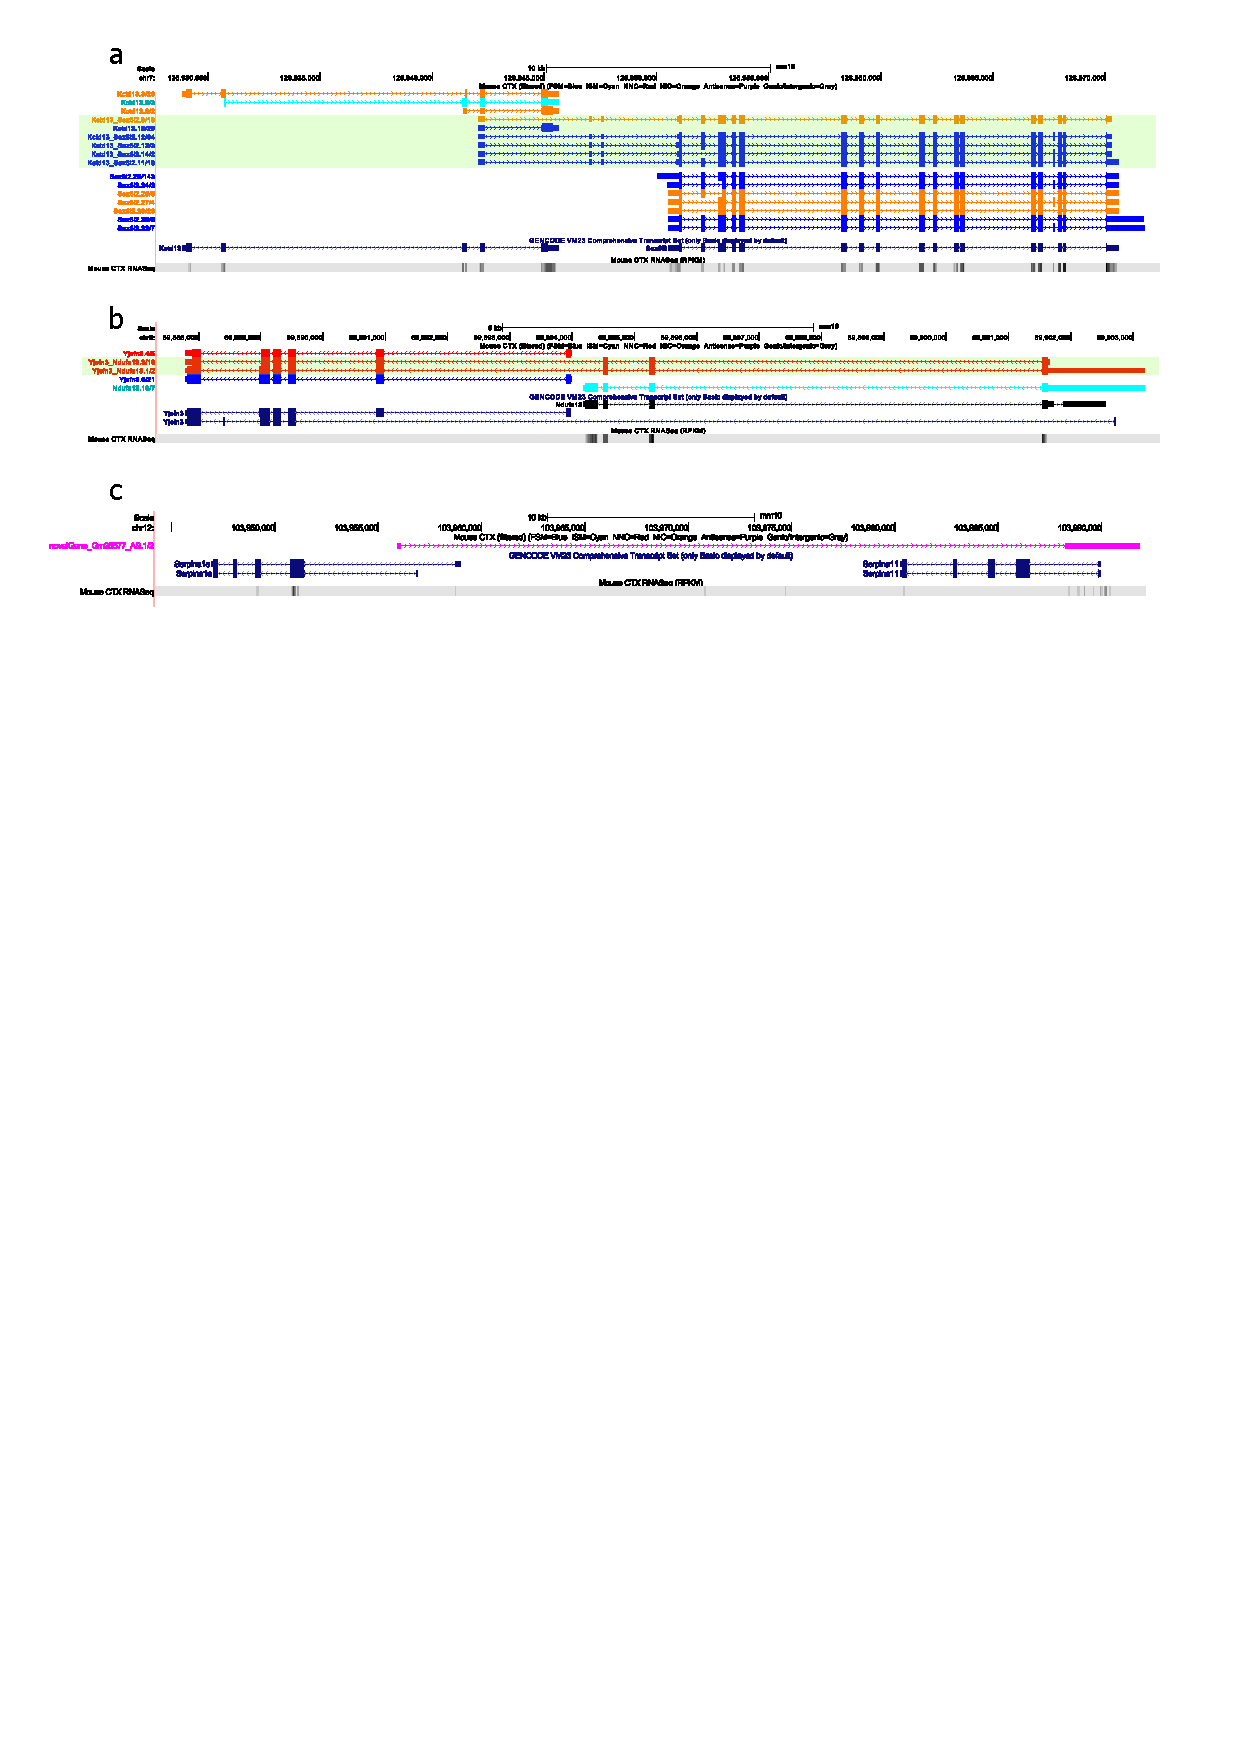
\includegraphics[page=1,trim={0 20cm 0 0},scale = 1.2]{Figures/FusionNovelGenes.pdf}
		\end{center}
		\vspace{1cm}
		\captionsetup{width=1.5\textwidth}
		\caption[Examples of fusion transcripts and novel genes identified in the mouse cortex]%
		{\textbf{Examples of fusion transcripts and novel genes identified in the mouse cortex.} Shown are UCSC genome browser tracks of \textbf{(A)} Five read-through “fusion” transcripts incorporating exons from \textit{Kctd13} (SZ-associated) and \textit{Sez6l2} (SZ-associated), \textbf{(B)} Two read-through “fusion” transcripts incorporating exons from \textit{Yjefn3} and \textit{Ndufa13} (SZ-associated), and \textbf{C)} a novel antisense transcript spanning across \textit{Serpina1e} and \textit{Serpina11} in the mouse cortex. Transcripts are coloured based on \textit{SQANTI2} classification categories (blue = FSM, cyan = ISM, red = NNC, orange = NIC). Fusion transcripts are boxed in green. SZ - Schizophrenia.}   
		\label{fig:isoseq_whole_novelfusion}
	\end{figure}
\end{landscape}


\subsection{Many transcripts map to long non-coding RNA genes}
Although the majority of transcripts (n = 43,450, 93.6\% of total transcripts) were classified as protein-coding by the presence of an open reading frame (ORF), a relatively large number of transcripts were annotated as encoding long non-coding RNAs (lncRNAs)\nomenclature{LncRNAs}{Long non-coding RNAs} (n = 1,141 transcripts associated with 734 genes). These lncRNA transcripts were shorter than non-lncRNA transcripts (lncRNA transcripts: mean length = 2.22kb, s.d = 1.36kb, range = 0.148kb - 8.49kb; non-lncRNA transcripts: mean length = 3.21kb, s.d = 1.68kb, range = 0.083kb - 15.9kb; W = 3.52 x 10\textsuperscript{7}, \textit{P} = 8.24 x 10\textsuperscript{-98}, \cref{fig:isoseq_whole_lncRNA}\textbf{A}), and contained fewer exons\cite{Statello2020} (W = 4.56 x 10\textsuperscript{7}, \textit{P} < 2.23 x 10\textsuperscript{-308}, \cref{fig:isoseq_whole_lncRNA}\textbf{B}) with a dramatic enrichment of mono-exonic molecules\cite{Kuo2017} (n = 273, 23.9\% of lncRNA transcripts) compared to non-lncRNA transcripts (n = 914, 2.02\% of non-lncRNA transcripts). They were also characterised by lower transcript expression than non-lncRNA transcripts \cite{Statello2020, Liu2016a} (W = 3.16 x 10\textsuperscript{7}, \textit{P} = 5.67 x 10\textsuperscript{-40}, \cref{fig:isoseq_whole_lncRNA}\textbf{C}), and detected with fewer isoforms (lncRNA transcripts: mean n = 1.55; non-lncRNA transcripts: mean n = 3.29; W = 7.40 x 10\textsuperscript{6}, \textit{P} = 5.76 x 10\textsuperscript{-107}, \cref{fig:isoseq_whole_lncRNA}\textbf{E}). A small proportion of these annotated lncRNA transcripts further contained a putative ORF (n = 153, 13.4\%, \cref{fig:isoseq_whole_lncRNA}\textbf{D}) supporting recent observations that some lncRNAs have potential protein coding capacity\cite{Kageyama2011}, although the majority of such ORFs are unlikely to code for proteins\cite{Guttman2013}; of note, these ORFs were shorter than those identified in non-lncRNA transcripts (non-lncRNA ORF: mean length = 139bp; lncRNA ORF: mean length = 519bp; W = 1.75 x 10\textsuperscript{7}, \textit{P} = 8.33 x 10\textsuperscript{-195}). 

\begin{figure}[htp]
	\begin{center}
		\includegraphics[page=7,trim={0 1cm 0 0},scale = 0.55]{Figures/IsoSeqWholeTranscriptome.pdf}
	\end{center}
	\captionsetup{width=0.95\textwidth}
	\caption[Characterisation of LncRNAs in the mouse cortex]%
	{\textbf{LncRNA transcripts were more lowly expressed and typically longer than non-lncRNA transcripts, despite containing fewer exons.} Shown are distributions of the \textbf{(A)} transcript length, \textbf{(B)} number of exons, \textbf{(C)} transcript expression, \textbf{(D)} open reading frame (ORF) length and the \textbf{(E)} number of isoforms annotated to lncRNAs and non-lncRNAs. LncRNAs – Long non-coding RNAs.}
	\label{fig:isoseq_whole_lncRNA}
\end{figure}

\subsection{AS strongly contributes to cortical isoform diversity}
\label{ch4_AS}
In total, 40,249 alternative splicing events were identified in known genes with AF (Alternative first exon) (n = 2,853 (31.9\%) associated with 6,476 (44.1\%) genes) and ES (Exon skipping, n = 8,686 (21.6\%) events associated with 4,570 (31.1\%) genes) being the most prevalent (\cref{fig:isoseq_whole_As_events}\textbf{A}). Splicing events and frequency were also compared between known and novel isoforms. Except for AF and AL, all the other splicing events, particularly intron retention, were more likely to be observed in novel isoforms. This highlights the power of Iso-Seq to recapitulate the usage of complex splicing events that would have otherwise been underestimated using RNA-Seq data (Fisher's Test, A3: \textit{P} = 7.78 x 10 \textsuperscript{–14}, odds ratio = 1.34; A5: \textit{P} = 1.21 x 10\textsuperscript{–13}, odds ratio = 1.45; IR: \textit{P} < 2.23 x 10\textsuperscript{–16}, odds ratio = 4.92; MX: \textit{P} = 4.18 x 10\textsuperscript{–11}, odds ratio = 1.81; ES: \textit{P} < 2.23 x 10\textsuperscript{–16}, odds ratio = 1.57, \cref{fig:isoseq_whole_As_events}\textbf{A}). For the majority of genes characterised by splicing, only 1 - 2 AS events were observed (n = 10,708, 81.8\% of AS genes, \cref{fig:isoseq_whole_As_events}\textbf{B}), suggesting that AS events are often mutually independent. 

\vspace{1cm}
\begin{figure}[!h]
	\begin{center}
		\includegraphics[page=5,trim={0 26cm 0 0},clip,scale = 0.55]{Figures/IsoSeqWholeTranscriptome.pdf}
	\end{center}
	\captionsetup{width=0.95\textwidth}
	\caption[Alternative splicing events from transcriptome profiling of the mouse cortex]%
	{\textbf{Alternative first is the most prevalent AS event, and novel isoforms were more likely to be characterised with complex AS events.} Shown are bar-plots of the \textbf{(A)} proportion of AS events in known genes, known and novel isoforms, and the \textbf{(B)} proportion of alternatively-spliced genes with varying number of splicing events. AF – Alternative first exon, AL – Alternative last exon, A5’ – Alternative 5’ splice site, A3’ – Alternative 3’ splice site, IR – Intron retention, MX – Mutually exclusive, ES – Exon skipping.}
	\label{fig:isoseq_whole_As_events}
\end{figure}


\subsection{Intron retention is associated with reduced expression and nonsense-mediated decay}
\label{ch4: IR}
Nonsense-mediated decay (NMD) acts to reduce transcriptional errors by degrading transcripts containing premature stop codons\cite{Hug2015} and is one mechanism by which intron retention can influence gene expression\cite{Pan2006} (described in \cref{intro:AS}). Overall, > 10\% of transcripts mapping to annotated genes were predicted to undergo NMD (NMD transcripts) characterized by the presence of an open reading frame and a coding sequence (CDS) end motif before the last junction (n = 6,014 (13.0\%) transcripts associated with 2,945 (20.3\%) of annotated genes). These NMD transcripts were less abundant than non-NMD transcripts (NMD transcripts: mean expression = 11.2 TPM, s.d =  85.0 TPM; non-NMD transcripts: mean expression = 23.1 TPM, s.d = 143.1 TPM; W = 8.72 x 107, \textit{P} = 6.15 x 10\textsuperscript{-156}).  NMD was particularly enriched among transcripts that contained an IR event (IR transcripts) and were also predicted to be protein-coding (n = 2,341 (36.2\%) IR transcripts associated with 1,380 (9.53\%) genes), and transcripts with both IR and predicted NMD were particularly lowly expressed (W = 7.50 x 10\textsuperscript{6}, \textit{P} = 1.67 x 10\textsuperscript{-42}, \cref{fig:isoseq_whole_IRNMD}\textbf{A}). Only a small number of genes had transcripts where IR and NMD were mutually exclusive (n = 277 genes, 1.91\%,
\cref{fig:isoseq_whole_IRNMD}\textbf{B}), providing additional support for the hypothesized relationship between these two transcriptional control mechanisms\cite{Ge2014}. 


\begin{figure}[!h]
	\begin{center}
		\includegraphics[page=6,trim={0 26cm 0 0},clip,scale = 0.55]{Figures/IsoSeqWholeTranscriptome.pdf}
	\end{center}
	\captionsetup{width=0.95\textwidth}
	\caption[Association of intron retention and nonsense-mediated decay]%
	{\textbf{Intron retention is associated with nonsense-mediated decay and reduced expression.} Shown is \textbf{(A)} a bar-plot of the expression of transcripts characterised with intron retention (IR) and nonsense-mediated decay (NMD), and \textbf{(B)} a Venn diagram of the number of genes associated with transcripts characterised with intron retention (IR), nonsense-mediated decay (NMD), or both (IR-NMD). As shown in Figure B, 1380 genes were associated with IR transcripts that were predicted for NMD, and 277 genes were associated with mutually exclusive IR transcripts and NMD transcripts. }
	\label{fig:isoseq_whole_IRNMD}
\end{figure}


\newpage
\section{Conclusions}
We used long-read isoform sequencing to characterize full-length cDNA sequences and generate a detailed map of alternative splicing in the mouse cortex. To our knowledge, this study represents the most comprehensive characterization of cortical isoform diversity yet undertaken. 

Several findings are particularly notable. First, we highlight that existing gene annotations are incomplete and that novel transcripts are likely to exist for a large proportion of expressed genes. Our data show examples of novel exons and even entire genes not currently annotated in existing databases. Second, we show that read-through transcripts (or gene fusion transcripts) occur naturally\cite{Mehani2020} and at detectable levels in the cortex. Although many of these fusion transcripts appear to be associated with NMD, some have the potential to be translated into proteins or may have a regulatory effect at the RNA level. Third, we are able to highlight the significant extent to which alternative splicing events contribute to isoform diversity in the cortex. In particular we show that IR is a relatively common form of AS in the cortex that is associated with reduced expression and NMD. Finally, our findings highlight the power of long-read sequencing approaches for transcriptional profiling. We show that transcriptional profiles generated using Iso-Seq reflect the cerebral cortex as expected, and our findings were validated using complementary approaches (i.e. RNA-Seq, and by comparison to existing genomic databases). Despite long-read sequencing often assumed to be less quantitative than standard short-read RNA sequencing methods\cite{Zhao2019}, we observed a strong correlation between expected and detected levels of ERCC spike-in control molecules, highlighting the power of Iso-Seq to accurately quantify the abundance of highly-expressed transcripts.

Our results should be interpreted in the context of several limitations. First, we profiled tissue from a relatively small number of mouse samples. Although rarefaction curves confirmed our sequencing dataset was close to saturation, we were unable to explore inter-individual variation in alternative splicing. Future work will aim to extend our analyses to larger numbers of samples to explore population-level variation in transcript abundance in the mouse cortex and differences associated with AD pathology. Second, despite the advantages of long-read sequencing approaches for the characterization of novel full-length transcripts, we implemented a stringent QC pipeline and undertook considerable filtering of our data. Many true transcripts from our final dataset, particularly lowly-expressed transcripts, are likely to have been filtered out. Our analyses are likely to represent an underestimation of the extent of RNA isoform diversity in the cerebral cortex. Future work will aim to sequence samples at a deeper coverage to explore gene-specific splicing differences associated with AD. Third, our analyses were performed on “bulk” cortex tissue containing a heterogeneous mix of neurons, oligodendrocytes and other glial cell-types. A recent study using a combination of long-read and single-cell sequencing identified cell-type-specific transcript diversity in the mouse hippocampus and prefrontal cortex\cite{Joglekar2021} (described in \cref{tab: longread_advancedstudies}). However, we were limited in exploring these differences in our data. Finally, although we explored the extent to which novel transcripts contained ORFs, the extent to which they are translated and contribute to cortical proteomic diversity is unknown.  

In summary, our data confirm the importance of alternative splicing and alternative first exon usage in the mouse entorhinal cortex, dramatically increasing transcriptional diversity and representing an important mechanism underpinning gene regulation in the brain. We highlight the power of long-read sequencing for completing our understanding of mouse gene annotation. The transcript level data is provided as a resource to the scientific community (http://genome.exeter.ac.uk/BrainIsoforms.html). 

%Although skipped exons are known to be the most common AS events in mouse, our data conversely suggests that splice variants from a single gene are predominantly generated through alternative first exons 
%Single cell analysis (\cite{Karlsson2017}) noted that alternative TSS and TTS variation in the first exon representing more than 70\% of splicing events,






